
%%%%%%%%%%%%%%%%%%%%%%%%%%%%%%%%%%%%%%%%%%%%%%%%%%%%%%%%%%%%%%%%%%%%%%%%%%%%%%%%%%%%%%%%%%
\begin{document}
\maketitle
%%%%%%%%%%%%%%%%%%%%%%%%%%%%%%%%%%%%%%%%%%%%%%%%%%%%%%%%%%%%%%%%%%%%%%%%%%%%%%%%%%%%%%%%%%

%%%%%%%%%%%%%%%%%%%%%%%%%%%%%%%%%%%%%%%%%%%%%%%%%%%%%%%%%%%%%%%%%%%%%%%%%%%%%%%%%%%%%%%%%%
\section{Mobiele Node}
%%%%%%%%%%%%%%%%%%%%%%%%%%%%%%%%%%%%%%%%%%%%%%%%%%%%%%%%%%%%%%%%%%%%%%%%%%%%%%%%%%%%%%%%%%

\begin{frame}[fragile]
\frametitle{Mobiele Node} 
\begin{itemize}
 \item Text
 \item More text
 \item More text again
\end{itemize}
\end{frame}

\note{Uitleg van kwinten, ook uitleg van doorsturen via Dash7 (of als iemand anders dit moet doen)}

%%%%%%%%%%%%%%%%%%%%%%%%%%%%%%%%%%%%%%%%%%%%%%%%%%%%%%%%%%%%%%%%%%%%%%%%%%%%%%%%%%%%%%%%%%
\section{Localisatie}
%%%%%%%%%%%%%%%%%%%%%%%%%%%%%%%%%%%%%%%%%%%%%%%%%%%%%%%%%%%%%%%%%%%%%%%%%%%%%%%%%%%%%%%%%%

\begin{frame} 
\frametitle{Localisatie}
  \begin{itemize}
  \item Text
  \item More text
  \item More text again
  \end{itemize}
\end{frame}

\note{Uitleg van Frederik, Dash7 localisatie en magnetometer}

%%%%%%%%%%%%%%%%%%%%%%%%%%%%%%%%%%%%%%%%%%%%%%%%%%%%%%%%%%%%%%%%%%%%%%%%%%%%%%%%%%%%%%%%%%
\section{Gateway}
%%%%%%%%%%%%%%%%%%%%%%%%%%%%%%%%%%%%%%%%%%%%%%%%%%%%%%%%%%%%%%%%%%%%%%%%%%%%%%%%%%%%%%%%%%

\subsection{Sensoren}

\begin{frame} 
\frametitle{Gateway}
  \begin{itemize}
  \item Sensoren \\
  Voeg een image toe van PCB me Aanduiding
  \pause
  \note{\begin{itemize}
		\item CO2 (CCS811): Maakt gebruik van de BCM2835-library, ook gebruikt voor de eerste taken rond de STM-bordjes
		\item Andere sensoren maken gebruik van de standaard I2C-library in Linux.
			\begin{enumerate}
				\item MPL3115, adres is 0x60: Bit 1-3 geven druk en 4-5 temperatuur
				\item SI7021, adres is 0x40: 
					\begin{itemize}
						\item commando 0xF3, leest temperatuur uit
						\item commando 0xF5, leest vochtigheid uit
					\end{itemize}
				\item MAG3310, magnetometer ook op sensorbord maar niet ge\"{i}mplementeerd in project.
			\end{enumerate}
		\end{itemize}}
	\item Sensorwaarden op MQTT topics
  \end{itemize}
\end{frame}

\note{\begin{itemize}
\item We hebben functies geschreven om alle data apart te lezen van de sensoren. Deze 		functies worden aangeroepen door een MAIN-functie. De gelezen waarden worden gefilterd (foute lezingen) en op verschillende MQTT Topics gezet 
	\begin{enumerate}
	\item rpi/temperature, rpi/humidity, rpi/pressure, rpi/airquality
	\end{enumerate}
\end{itemize}}

\subsection{LED Visualisatie}

\begin{frame} 
\frametitle{Gateway}
  \begin{itemize}
  \item LED Visualisatie: \\
  \begin{enumerate}
  	\item Profielen
  	\item CO\textsubscript{2} en Temperatuur Niveau
  \end{enumerate}
  	\begin{center}
  		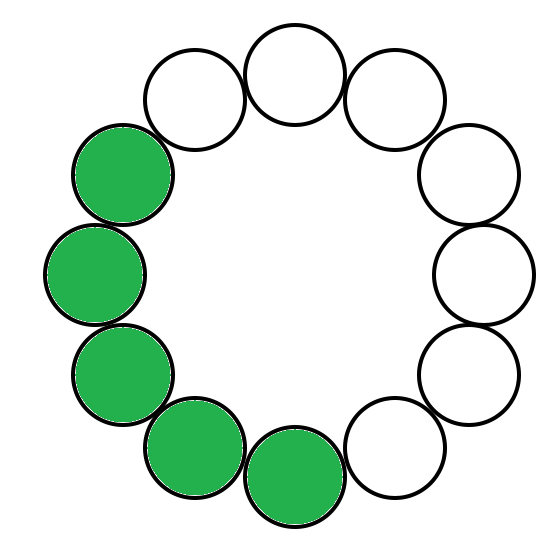
\includegraphics[width=.5\textwidth]{images/LEDlow.png}
  		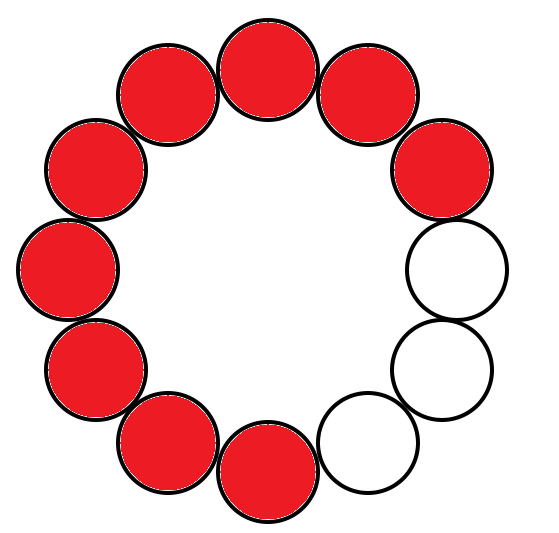
\includegraphics[width=.5\textwidth]{images/LEDhigh.png}
	\end{center}
  \end{itemize}
\end{frame}

\note{\begin{itemize}
\item LEDs worden aangestuurd via een python script. Dit script wordt aangeroepen via het algemeen sensorscript, geschreven in C. 
\item Een script leest temperatuur/CO2 waarden uit, steekt ze in een variabele van Python en runt het script. De kleur geeft de luchtkwaliteit weer (Groen = goed, rood = slecht), het aantal ledjes geeft de temperatuur weer.
\item Als er iemand binnenkomt, nemen de leds een preference color aan a.d.h.v. de id van RFID chip. De kleur word geoverride bij de volgende temperatuur/co2-meting.
\end{itemize}}

%%%%%%%%%%%%%%%%%%%%%%%%%%%%%%%%%%%%%%%%%%%%%%%%%%%%%%%%%%%%%%%%%%%%%%%%%%%%%%%%%%%%%%%%%%
\section{openHAB}
%%%%%%%%%%%%%%%%%%%%%%%%%%%%%%%%%%%%%%%%%%%%%%%%%%%%%%%%%%%%%%%%%%%%%%%%%%%%%%%%%%%%%%%%%%

\begin{frame} 
\frametitle{openHAB}
  \begin{itemize}
  \item Text
  \item More text
  \item More text again
  \end{itemize}
\end{frame}

\note{Uitleg van Bernd, implementatie in openHAB, tegelijk met demo mss}

%%%%%%%%%%%%%%%%%%%%%%%%%%%%%%%%%%%%%%%%%%%%%%%%%%%%%%%%%%%%%%%%%%%%%%%%%%%%%%%%%%%%%%%%%%
\section{Demo}
%%%%%%%%%%%%%%%%%%%%%%%%%%%%%%%%%%%%%%%%%%%%%%%%%%%%%%%%%%%%%%%%%%%%%%%%%%%%%%%%%%%%%%%%%%

\begin{frame} 
\frametitle{Demo}
  \begin{itemize}
  \item Text
  \item More text
  \item More text again
  \end{itemize}
\end{frame}

%%%%%%%%%%%%%%%%%%%%%%%%%%%%%%%%%%%%%%%%%%%%%%%%%%%%%%%%%%%%%%%%%%%%%%%%%%%%%%%%%%%%%%%%%%
\end{document}
%%%%%%%%%%%%%%%%%%%%%%%%%%%%%%%%%%%%%%%%%%%%%%%%%%%%%%%%%%%%%%%%%%%%%%%%%%%%%%%%%%%%%%%%%%